%Copyright 2013-2014 Stephen Kraemer

\documentclass{letter}

\usepackage[colorlinks=true, urlcolor=blue]{hyperref}
\usepackage{grffile}
\usepackage{geometry}

%margins
\newgeometry{left=20mm,right=20mm,top=20mm, bottom=20mm}

%get rid of headers/footers (i.e. no page numbers)
\pagestyle{empty}

\begin{document}

{\Huge\bf Stephen Kraemer} \hfill
\begin{tabular}{r}
  \href{https://github.com/straemer}{github.com/straemer} \\
  (226) 606-4052 \\
  \href{mailto:sbkraeme@uwaterloo.ca}{sbkraeme@uwaterloo.ca}
\end{tabular}

%horizontal line
\vskip 2pt
\hrule

{\large\bf SUMMARY OF QUALIFICATIONS}
\begin{itemize}
  \item Proficient in programming in a multi-threaded environment
  \item Familiar with protocols throughout the network stack
  \item Attentive to detail in both writing software and in integrating with existing code
  \item Experience working in performance sensitive code
\end{itemize}

\vskip 2pt

{\bf Programming Languages and Tools}

%minipages = magic to make side-by-side columns
\begin{minipage}{0.35\textwidth}
  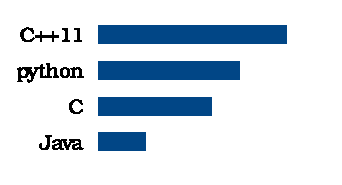
\includegraphics{programming_languages.eps}
\end{minipage}
\begin{minipage}{0.65\textwidth}
  \begin{itemize}
    \item Operating Systems: Linux (day-to-day Ubuntu and Arch Linux user)
    \item Version Control: git, svn, perforce
    \item Embedded Systems: Arduino, Raspberry Pi
    \item Other Tools: gdb, valgrind, make, LaTeX, emacs, wireshark
  \end{itemize}
\end{minipage}

%horizontal line
\vskip 2pt
\hrule
{\large\bf WORK EXPERIENCE}

{\bf Oracle,} Endeca Server Team, {\sl Boston, MA} \hfill Apr-Aug 2013 \\
{\sl Software Developer}
\begin{itemize}
  \item Worked on performance and scaling team of an analytical database.
  \item Increased query performance by up to 10\% by finding and fixing a bug in cache eviction algorithm.
\end{itemize}
{\bf Technical Environment:} C++11, python, Linux, Windows, multi-threaded programming, make, gdb, valgrind, svn, git

{\bf Autodesk,} Alias Team, {\sl Toronto, ON} \hfill Aug-Dec 2012 \\
{\sl Software Developer}
\begin{itemize}
  \item Developed software for a 3D modelling program.
  \item Completely redesigned the printing work-flow, integrating Qt into a product that did not previously use it.
\end{itemize}
{\bf Technical Environment:} C++, Objective-C, Windows, OS X, multi-threaded programming, jam (Just Another Make), gdb, perforce, Qt

{\bf Avvasi Inc,} Packet Processing Team, {\sl Waterloo, ON} \hfill Jan-Apr 2012 \\
{\sl Software Developer}
\begin{itemize}
  \item Worked on product to analyze and improve video streaming over a large-scale network.
  \item Ported RTMP and RTSP parsers from an older product to a newer one.
\end{itemize}
{\bf Technical Environment:} C++11, Linux, multi-threaded programming, network programming, gcc, make, gdb, valgrind, svn, ssh, wireshark

%horizontal line
\vskip 2pt
\hrule

\newpage
{\large\bf EDUCATION}

{\bf Candidate for Bachelor of Applied Science} \hfill Sept 2009 - Apr 2014 \\
Mechatronics Engineering \hfill University of Waterloo, ON

{\bf Fourth Year Design Project} - \href{http://www.casesensitive.ca}{www.casesensitive.ca} \hfill Sept 2013 - Apr 2014
\begin{itemize}
  \item Designed a ``smart'' suitcase that tracks its position, detects mishandling, and weighs itself; reporting this information to a smartphone.
  \item Software lead in a team of four.
\end{itemize}
{\bf Technical Environment:} C++, PHP, Java, Arduino, Android, Raspberry Pi, network programming, wireshark

%horizontal line
\vskip 2pt
\hrule
{\large\bf INTERESTS}
\begin{itemize}
  \item Heavy metal music
  \item Video Games: Minecraft, Pokemon, Zelda
  \item University of Waterloo Engineering Society member
\end{itemize}

\end{document}
